%%%%%%%%%%%%%%%%%%%%%%%%%%%%%%%%%%%%%%%%%%%%%%%%%%%%%%%%%%%%%%%%%%%%%%%%%%%%%%%%
\chapter{Разработка метода программной редукции}
%%%%%%%%%%%%%%%%%%%%%%%%%%%%%%%%%%%%%%%%%%%%%%%%%%%%%%%%%%%%%%%%%%%%%%%%%%%%%%%%
В соответствии с поставленной задачей необходимо разработать метод редукции программ на языке Kotlin.
Разрабатываемый метод является гибридным и состоит из следующих этапов: 
\begin{itemize}
	\item предварительное упрощение проекта;
	\item слайсинг;
	\item трансформации над текстовым представлением программы;
	\item трансформации над синтаксическим деревом~(СД);
	\item иерархический дельта дебаггинг.
\end{itemize}

\begin{figure}
\center{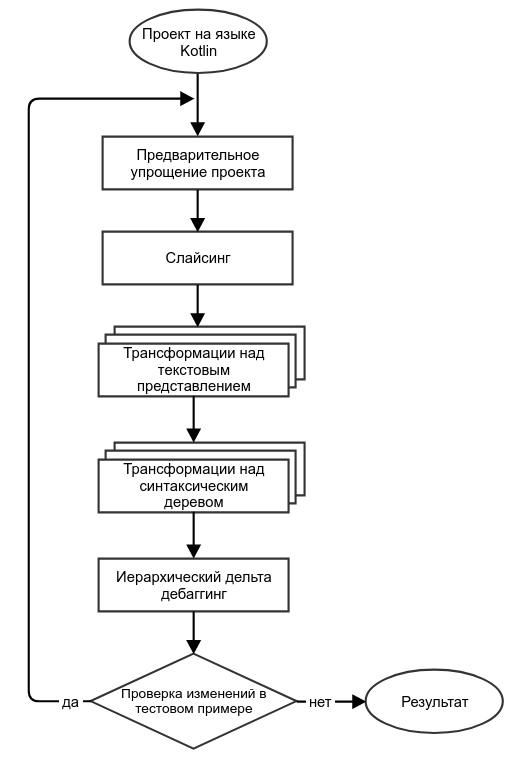
\includegraphics[width=0.75\linewidth]{fig/scheme}}
\caption{\label{scheme}Схема работы метода программной редукции}
\end{figure}
Схема работы метода представлена на рисунке~\ref{scheme}. Приведенные компоненты запускаются друг за другом в цикле до того момента, как тестовый пример не перестанет изменяться. Для обеспечения безопасности преобразований, после применения каждой трансформации производится проверка воспроизведения ошибки на полученном тестовом примере. Если ошибка не воспроизводится, то производится откат тестового примера в предыдущее состояние и переход к следующей трансформации.
Для каждого этапа программной редукции в данном разделе описан алгоритм работы и обоснована его актуальность.

%%%%%%%%%%%%%%%%%%%%%%%%%%%%%%%%%%%%%%%%%%%%%%%%%%%%%%%%%%%%%%%%%%%%%%%%%%%%%%%%
\section{Проверка воспроизведения ошибки}\label{errorscheck}
%%%%%%%%%%%%%%%%%%%%%%%%%%%%%%%%%%%%%%%%%%%%%%%%%%%%%%%%%%%%%%%%%%%%%%%%%%%%%%%%
Изначально необходимо решить проблему проверки воспроизведения ошибки. Проблема состоит в том, что часто сообщения об одной и той же ошибке могут достаточно сильно различаться. Например, сообщение об ошибке компилятора может содержать часть сгенерированного байт-кода, который в процессе редукции может изменяться от трансформации к трансформации.

Существует 2 способа решения данной проблемы. Первый --- при известном формате сообщения об ошибке производить выделение необходимой информации. Данный способ хорошо применим к компиляторным сбоям, где сообщение об ошибке имеет определенный формат. Пример такого сообщения приведен на рисунке~\ref{ex:error}. Как видно из рисунка, из сообщения легко можно выделить тип ошибки и ее местоположение.
%
\begin{figure}
\center{
\begin{lstlisting}
Error:Kotlin: [Internal Error] org.jetbrains.kotlin.codegen.CompilationException: Back-end (JVM) Internal error: wrong code generated
org.jetbrains.kotlin.codegen.CompilationException Back-end (JVM) Internal error: Couldn't transform method node:
test ()V:
   L0
    LINENUMBER 2 L0
   L1
    POP
   L2
...
Cause: AFTER mandatory stack transformations: incorrect bytecode
Element is unknownThe root cause was thrown at: MethodVerifier.kt:28
File being compiled at position: (1,1) in Main.kt
...
\end{lstlisting}
\caption{\label{ex:error}Пример сообщения об ошибке для компилятора языка Kotlin}
}
\end{figure} 

Второй способ --- сравнивать непосредственно сообщения об ошибке. Для решения этой задачи подходит разностный алгоритм, предложенный Майерсом~\cite{myers1986ano}. Алгоритм принимает два файла и генерирует инструкции для превращения одного файла в другой. Инструкции могут быть двух типов: удаление из первого файла и вставка во второй. Количество таких конструкций должно быть минимально возможным. Данная задача эквивалентна задаче поиска наибольшей общей подпоследовательности~(НОП). Для нахождения НОП удобнее всего построить специальный граф редактирования. Пусть первый файл $A = a_1...a_N$ и второй файл $B = b_1...b_M$~--- последовательности длиной $N$ и $M$ соответственно. Граф редактирования для $A$ и $B$ имеет узел в каждой точке решетки $(x, y)$, где $x \in [0, N]$, и $y \in [0, M]$. Узлы графа соединены горизонтальными, вертикальными и диагональными направленными ребрами. Горизонтальные ребра соединяют каждый узел с правым соседом, вертикальные --- с соседом снизу. Если $a_x = b_y$, то строится диагональное ребро, соединяющее узлы $(x-1, y-1)$ и $(x, y)$. После построения графа задача сводится к поиску пути с наибольшим количеством диагональных ребер.
На рисунке~\ref{ex:lcs} приведен пример графа редактирования и такого пути для последовательностей $A = abcabba$ и $B = cbabac$ из статьи~\cite{myers1986ano}. Наибольшей общей последовательностью является подпоследовательность вершин, в которые приходят диагональные ребра. Для данного примера это будет последовательность $caba$. После нахождения НОП можно вычислить коэффициент схожести строк, поделив сумму длин различающихся последовательностей на сумму длин совпадающих. Далее на основе сравнения полученного коэффициента с заданной константой делается вывод о том, считаются ошибки совпадающими или нет.

\begin{figure}	
		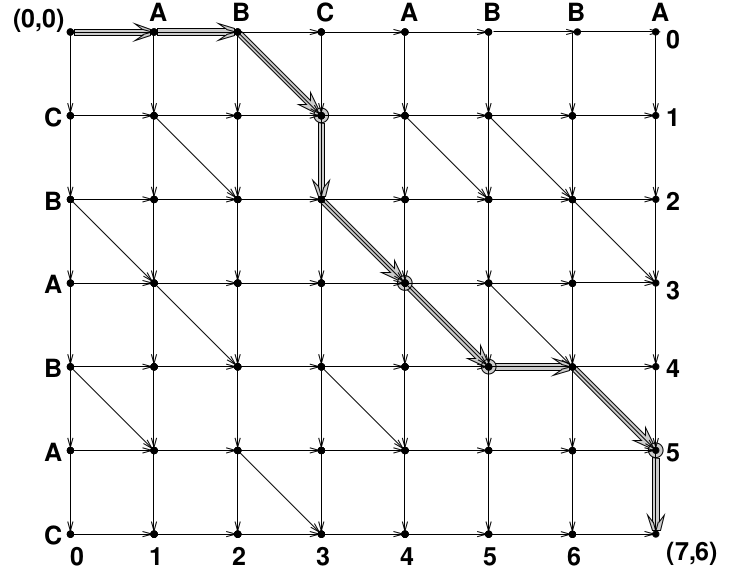
\includegraphics[width=0.99\linewidth]{fig/lcsexample} 
		\caption{\label{ex:lcs}Граф редактирования и НОП для последовательностей $A = abcabba$ и $B = cbabac$}
\end{figure}
В итоге, если сообщение об ошибке подходит под заданный шаблон, то должен применяться первый способ. Если же тип и локацию сбоя выделить не удается, то применяется второй способ. Константа, с которой сравнивается коэффициент схожести, была подобрана экспериментально и равна~1.5.

%%%%%%%%%%%%%%%%%%%%%%%%%%%%%%%%%%%%%%%%%%%%%%%%%%%%%%%%%%%%%%%%%%%%%%%%%%%%%%%%
\section{Предварительное упрощение проектов}
%%%%%%%%%%%%%%%%%%%%%%%%%%%%%%%%%%%%%%%%%%%%%%%%%%%%%%%%%%%%%%%%%%%%%%%%%%%%%%%%
Современные программы имеют множество сложных внутренних связей, поэтому зачастую удаление нерелевантной ошибке информации из целевого файла становится невозможным, поскольку эта информация используется в другой части проекта. Для решения данной проблемы выполняется предварительное упрощение проекта --- редукция связанных с целевым (содержащим ошибку) файлов. Для формирования выборки файлов для упрощения используются списки импортирований\footnote{https://kotlinlang.org/docs/reference/packages.html}. Каждая позиция в таком списке содержит все конструкции, которые могут быть использованы из другого пакета. 

В списке импортирований для языка программирования Kotlin может использоваться символ <<*>> --- знак обобщения импортирования. Это означает то, что из указанного пакета импортируются все возможные конструкции. В разработанном алгоритме <<*>> заменяется на все возможные импортирования из указанного пакета. Например, если в пакете \texttt{a} содержатся классы \texttt{A} и \texttt{B}, а в пакете \texttt{b} содержится импортирование \texttt{import a.*}, то оно будет преобразовано в \texttt{import a.A} и \texttt{import a.B}.

Разработанный алгоритм сначала получает список всех конструкций, которые могут быть включены из целевого пакета с ошибкой, затем рекурсивно проходит по всем файлам с целью поиска импортирований из целевого. Попутно строится дерево зависимостей, в котором каждый узел --- это файл, а его глубина --- порядок зависимости от целевого. Стоит отметить, что при построении дерева избегаются все циклические зависимости.

Например, пусть \texttt{A} --- целевой файл с ошибкой. В файлы~\texttt{B} и~\texttt{C} импортируются конструкции из \texttt{А}, а в \texttt{D} --- из \texttt{B}. Дерево зависимостей для примера приведено на рисунке~\ref{ex:tree}. 
%
\begin{figure}
\center{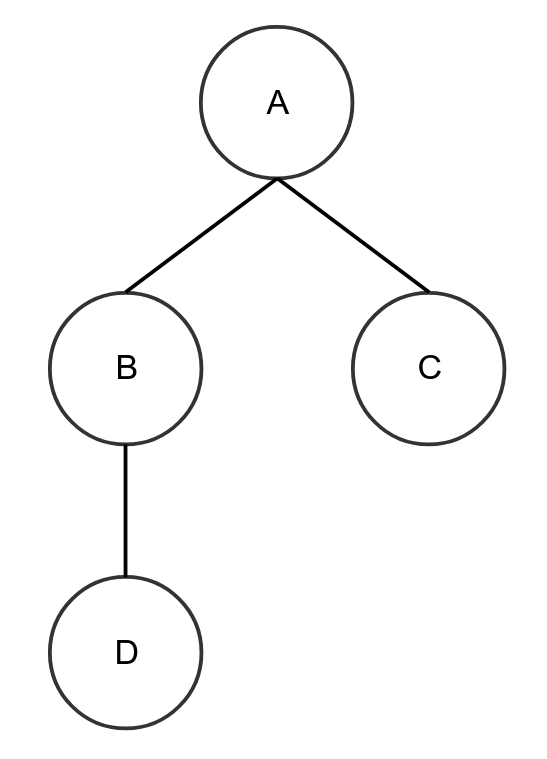
\includegraphics[width=0.3\linewidth]{fig/treeexample}}
\caption{\label{ex:tree}Пример построения дерева зависимостей}
\end{figure}
%
После построения дерева последовательно, начиная с наибольшей глубины, производится запуск упрощающих трансформаций над каждым узлом в дереве. Ниже приведен список трансформаций, каждая из которых подробно описана далее в этом разделе:
%
\begin{itemize}
	\item упрощение функций и свойств;
	\item трансформации над текстовым представлением;
	\item удаление пустых управляющих конструкций;
	\item удаление неиспользуемых импортирований.
\end{itemize}

%%%%%%%%%%%%%%%%%%%%%%%%%%%%%%%%%%%%%%%%%%%%%%%%%%%%%%%%%%%%%%%%%%%%%%%%%%%%%%%%
\section{Программный срез}\label{slicingalg}
%%%%%%%%%%%%%%%%%%%%%%%%%%%%%%%%%%%%%%%%%%%%%%%%%%%%%%%%%%%%%%%%%%%%%%%%%%%%%%%%
Алгоритмы слайсинга были описаны в разделе~\ref{slicing}. Ввиду простоты реализации и эффективности работы было решено реализовать обратный статический срез над синтаксическим деревом. Главной проблемой применения слайсинга для задачи программной редукции является обязательность наличия точной локации причины ошибки.
Программный срез производится на следующих уровнях:
\begin{itemize}
	\item уровень классов;
	\item уровень функций;
	\item уровень выражений.
\end{itemize}

%%%%%%%%%%%%%%%%%%%%%%%%%%%%%%%%%%%%%%%%%%%%%%%%%%%%%%%%%%%%%%%%%%%%%%%%%%%%%%%%
\subsection{Слайсинг на уровне классов и функций}
%%%%%%%%%%%%%%%%%%%%%%%%%%%%%%%%%%%%%%%%%%%%%%%%%%%%%%%%%%%%%%%%%%%%%%%%%%%%%%%%
Слайсинг на уровне функций работает следующим образом. Из целевой~(содержащей причину программной ошибки) функции производится рекурсивный обход всех вызовов из нее других функций и строится дерево использования. Далее функции, не входящие в построенное дерево, удаляются из файла. Аналогично работает срез на уровне классов. Пример слайсинга на уровне функций представлен на рисунке~\ref{funslicing}.
%
\begin{figure}[]
\centering
\begin{subfigure}[t]{\linewidth}
	\begin{lstlisting}
		fun funWithBug() {
			fun1()
		}
		
		fun fun1(){
			fun2()		
		}
		
		fun fun2(){}
		fun fun3(){}
	\end{lstlisting}
	\caption{Исходный код}
\end{subfigure}
\begin{subfigure}[t]{\linewidth}
	\begin{lstlisting}
		fun funWithBug() {
			fun1()
		}
		
		fun fun1(){
			fun2()		
		}
		
		fun fun2(){}
	\end{lstlisting}
	\caption{Результат слайсинга}
\end{subfigure}
	\caption{\label{funslicing}Пример слайсинга на уровне функций}
\end{figure}

%%%%%%%%%%%%%%%%%%%%%%%%%%%%%%%%%%%%%%%%%%%%%%%%%%%%%%%%%%%%%%%%%%%%%%%%%%%%%%%%
\subsection{Внутрипроцедурный слайсинг}
%%%%%%%%%%%%%%%%%%%%%%%%%%%%%%%%%%%%%%%%%%%%%%%%%%%%%%%%%%%%%%%%%%%%%%%%%%%%%%%%
Алгоритм внутрипроцедурного слайсинга приведен на рисунке~\ref{alg:interproceduralslicing}.
%
\begin{figure}
\textbf{ВХОД:} $line$ - номер строки, содержащей ошибку  \\
\textbf{ВХОД:} $funTree$ - синтаксическое дерево, представляющее целевую функцию \\
\textbf{ВЫХОД:} $funTree$ - редуцированное синтаксическое дерево \\
\begin{algorithmic}[1]
\STATE $curLine \leftarrow lastLine$
\WHILE{$curLine != line$} 
	\STATE $\text{deleteLine}(funTree, curLine)$
	\STATE $curLine \leftarrow curLine - 1$
\ENDWHILE
\STATE $monitoringElems \leftarrow \text{parseLine}(line)$
\STATE $curLine \leftarrow curLine - 1$
\WHILE{$curLine != firstLine$} 
	\IF{$\text{dependsOn}(curLine, monitoringElems)$} 
		\STATE $monitoringElems \leftarrow monitoringElems + \text{parseLine}(curLine)$ 
	\ELSE 
		\STATE $\text{deleteLine}(funTree, curLine)$ 
	\ENDIF
\ENDWHILE
\RETURN $funTree$
\end{algorithmic}
\caption{\label{alg:interproceduralslicing}Алгоритм внутрипроцедурного слайсинга}
\end{figure}
%
Входной информацией для алгоритма внутрипроцедурного слайсинга является номер строки, содержащей ошибку, и синтаксическое дерево, представляющее целевую функцию. В алгоритме производится обратный обход этой функции. До момента попадания в строку с ошибкой производится удаление всех выражений. Далее выделяются все переменные, содержащиеся в заданной строке --- они и будут являться критерием среза. При дальнейшем обходе функции в каждой строке производится проверка: влияют ли переменные из этой строки на переменные из критерия. Если влияют, то они добавляются к критерию, если нет --- производится удаление строки. Пример работы внутрипроцедурного слайсинга был приведен ранее в разделе~\ref{slicing}.

%%%%%%%%%%%%%%%%%%%%%%%%%%%%%%%%%%%%%%%%%%%%%%%%%%%%%%%%%%%%%%%%%%%%%%%%%%%%%%%%
\section{Трансформации над текстовым представлением программы}
%%%%%%%%%%%%%%%%%%%%%%%%%%%%%%%%%%%%%%%%%%%%%%%%%%%%%%%%%%%%%%%%%%%%%%%%%%%%%%%%
Трансформации над текстовым представлением программы появились из-за того, что некоторые трансформации из соображений эффективности нецелесообразно производить над синтаксическим деревом. Примером такой трансформации может быть удаление какой-либо части текста, изменение по шаблону и т.д. Ниже приведено описание сформированных трансформаций над текстовым представлением программы.

\paragraph{Удаление текста внутри сбалансированной пары скобок.}
Скобки в языке программирования Kotlin могут быть 4-х видов: фигурные, круглые, квадратные и треугольные, но удаление текста имеет смысл только для фигурных и круглых скобок. Данная трансформация находит все сбалансированные скобки в программе и пытается удалить весь текст внутри. В случае успешного воспроизведения ошибки с новым текстом программы данная трансформация применяется, в противном случае все возвращается обратно и производится переход к другой паре сбалансированных скобок. Часто в результате редукции появляются лишние пары скобок, поэтому данную трансформацию целесообразно дополнить функциональностью для их удаления. В качестве дополнительной может быть реализована трансформация, удаляющая текст между каждой парой точек. Таким образом может быть удален лишний вызов функции. Например \texttt{item.fun1.fun2} преобразуется в \texttt{item.fun2}.

\paragraph{Замена текста.}
Данные трансформации могут быть трех видов:
%
\begin{itemize}
	\item замена текста, подходящего под шаблон, например, <<1294>> на~<<0>>; 
	\item замена части текста, подходящего под шаблон, на другой, например <<\texttt{i = i + 1}>> на~<<\texttt{i++}>>;
	\item применение к тексту, подходящему под шаблон, другого шаблона, например <<\texttt{a + b + c + d}>> преобразуется в~<<\texttt{a + b}>>.
\end{itemize}
%
Ниже приведен список разработанных шаблонов и их замен:
%
\begin{itemize}
	\item замена арифметических операторов \texttt{+=} на \texttt{=};
	\item замена \texttt{while} на \texttt{if};
	\item замена целочисленных констант на 0;
	\item замена строковых констант на пустые;
	\item замена типов на целочисленный;
	\item упрощение бинарных операций.
\end{itemize}
%
На рисунке~\ref{ex:peephole} приведен пример применения трансформаций над текстовым представлением программы.
%
\begin{figure}[]
\centering
\begin{subfigure}[t]{\linewidth}
\begin{lstlisting}
fun f() {
    var a = 124125125
    val b = a + 1
    val c = 1.1
    var d: Double
    while (a.toDouble() != c) {
        d = a * b * c
        a += 1
    }
    println("a = $a")
}
\end{lstlisting}
\caption{Исходный код}
\end{subfigure}
\begin{subfigure}[t]{\linewidth}
\begin{lstlisting}
fun f() {
    var a = 0
    val b = a + 1
    val c = 0.0
    var d: Double
    if (a.toDouble() != c) {
        d = a * b
        a++
    }
    println("")
}
\end{lstlisting}
\caption{Результат применения трансформаций}
\end{subfigure}
\caption{\label{ex:peephole}Пример применения трансформаций над текстовым представлением программы}
\end{figure}

%%%%%%%%%%%%%%%%%%%%%%%%%%%%%%%%%%%%%%%%%%%%%%%%%%%%%%%%%%%%%%%%%%%%%%%%%%%%%%%%
\section{Трансформации над синтаксическим деревом}
%%%%%%%%%%%%%%%%%%%%%%%%%%%%%%%%%%%%%%%%%%%%%%%%%%%%%%%%%%%%%%%%%%%%%%%%%%%%%%%%
После трансформаций над текстовым представлением был сформирован набор трансформаций над~СД. СД в качестве редактируемого представления программы было выбрано из-за сложности проведения сформированных трансформаций над текстовым представлением и достаточности для этого информации, содержащейся в нем. Ниже приведено краткое описание сформированных в результате исследований трансформаций.

\paragraph{Удаление комментариев.} Часто программа содержит большое количество комментариев, которые являются нерелевантной информацией по отношению к программной ошибке, поэтому производится их удаление.

\paragraph{Упрощение элвис-оператора.}
Если имеется ссылка, которая может принимать значение \texttt{null}, можно провести проверку этой ссылки и использовать ее, либо использовать значение, которое не может принимать значение \texttt{null}: \texttt{val a = if (b != null) b else c}.
Аналогом такому if-выражению является элвис-оператор \texttt{?:} --- \texttt{val a = b ?: c}.
Данный оператор можно попытаться заменить на его правую часть. Например, выражение \texttt{val a = b ?: c} заменится на \texttt{val a = c}.

\paragraph{Удаление пустых управляющих инструкций.} Если какая-нибудь управляющая инструкция, например: \texttt{if}, \texttt{for}, \texttt{try}, \texttt{when} --- не содержит тела, то ее можно попытаться удалить.

\paragraph{Удаление унаследованных свойств и функций.} При редукции программ, реализующих объектно-ориентированную методологию, часто представляется невозможным удалить нерелевантную ошибке информацию из-за внутренних связей~(наследование и т.д.); но в некоторых случаях эти связи можно попытаться упростить. Данная трансформация рекурсивно проходит по всем родителям класса, в котором содержится ошибка, и удаляет поля с одинаковыми именами. Пример трансформации приведен на рисунке~\ref{ex:inh}.
%
\begin{figure}
\centering
\begin{subfigure}[t]{\linewidth}
\begin{lstlisting}
interface A {
    fun f()
}

open class B : A {
    override fun f() {}
}

class ClassWithBug : B() {
    override fun f() {}
    fun a() {}
}
\end{lstlisting}
\caption{Исходный код}
\end{subfigure}
\begin{subfigure}[t]{\linewidth}
\begin{lstlisting}
interface A {

}

open class B : A {

}

class ClassWithBug : B() {
    fun a() {}
}
\end{lstlisting}
\caption{Результат применения трансформации}
\end{subfigure}
\caption{\label{ex:inh}Пример работы трансформации для упрощения внутренних связей}
\end{figure}

\paragraph{Удаление аргументов функции.} В результате применения различных методов редукции аргументы функции часто становятся неиспользуемыми. Для их удаления необходимо найти все вызовы данной функции и одновременно удалить аргумент из функции и всех ее вызовов. Но в программе могут иметься другие функции с таким же названием и даже сигнатурой, поэтому для каждого вызова необходимо проверять тип аргументов и пакет, откуда вызываемая функция импортируется.

\paragraph{Удаление значений из списка родительских классов.} В процессе редукции наследование часто становится неиспользуемым. По этой причине в списке родительских классов каждый такой класс можно попытаться удалить.

\paragraph{Удаление неиспользуемых импортирований и переводов строк.} При редукции многие импортирования часто становятся неиспользуемыми, и их можно удалить. Также при редукции могут оставаться переводы строк, усложняющие читаемость результирующего кода, которые также удаляются.

\paragraph{Замена возвращаемого значения функции на константу.} Если функция имеет стандартный возвращаемый тип, например, \texttt{Int} или \texttt{String}, то правую часть оператора возврата \texttt{return} можно попытаться заменить на константное значение. Например, если функция имеет возвращаемый тип \texttt{Int}, то можно попытаться заменить правую часть всех операторов \texttt{return} на 0.

\paragraph{Замена типа возвращаемого значения функции на Unit.} Функция, не возвращающая никакого значения, в языке программирования Kotlin имеет тип \texttt{Unit}~(аналог \texttt{void} в Java). Стоит отметить, что тип возвращаемого значения \texttt{Unit} может быть опущен. Трансформация пытается заменить тип возвращаемого значения функции на \texttt{Unit} и удалить из нее все операторы возврата \texttt{return}.

\paragraph{Упрощение конструктора класса.} В результате редукции параметры из конструктора класса могут становиться неиспользуемыми. В этом случае их можно удалить, для этого необходимо удалить неиспользуемый аргумент непосредственно из конструктора и из всех его вызовов.

\paragraph{Упрощение цикла for.} Данная трансформация делает попытку вынести из цикла \texttt{for} его тело. В документации языка Kotlin описано, что цикл \texttt{for} позволяет проходить по всем элементам объекта, обладающего внутренней или внешней функцией \texttt{iterator()}, возвращаемый тип которой обладает внутренней или внешней функцией \texttt{next()} и \texttt{hasNext()}. Поэтому в случае использования в теле цикла его параметра необходимо создать свойство, левая часть которого будет этим параметром, а правая --- вызовом функций \texttt{iterator()} и \texttt{next()} у объекта, по которому производится итерация. Например, для цикла \texttt{for (item in collection) \{ ... \}} необходимо создать свойство \texttt{val item = collection.iterator().next()} и далее подставить его тело.

\paragraph{Упрощение функций и свойств.} Данная трансформация пытается заменить тела всех функций и правую часть всех свойств на вызов специальной функции \texttt{TODO()}, при обращении бросающей исключение \texttt{NotImplementedError}. Функция \texttt{TODO()} имеет возвращаемый тип \texttt{Nothing} --- специальный тип в языке Kotlin, который наследуется от всех остальных типов, не может иметь экземпляров и должен всегда указываться явно. Поэтому если функция или свойство имеет неуказанный явно возвращаемый тип, то его необходимо указать, так как иначе возвращаемым типом функции неявно станет \texttt{Nothing}, что запрещено компилятором.

\paragraph{Упрощение оператора \texttt{if}.} Данная трансформация пытается заменить оператор \texttt{if} на какую-либо его ветку. Необходимо различать в условии оператора сравнение переменной с каким-либо значением (\texttt{if (i == 0)}) и сравнение с каким-либо типом при помощи оператора \texttt{is} (\texttt{if (item is Type)}). Во втором случае возможно появление умных приведений\footnote{https://kotlinlang.org/docs/reference/typecasts.html}, так как компилятор следит за \texttt{is}-проверками для неизменяемых значений и вставляет приведения автоматически, там, где они нужны. Поэтому необходимо вручную приводить переменную из условия к типу, с которым она сравнивается для \texttt{true}-ветки. Для этого необходимо использовать оператор~\texttt{as} (\texttt{item as Type}).

\paragraph{Упрощение унаследованных свойств.} Данная трансформация направлена на упрощение унаследованных свойств. Сначала строится дерево, отражающее все родительские связи между классами. Если класс, в котором содержится причина отказа программы, переопределяет абстрактные свойства из родительского класса, их можно попытаться удалить. Для этого производится обход дерева, начиная с целевого класса, собираются все абстрактные наследованные свойства, и, в случае успешного воспроизведения ошибки, у этих свойств удаляется модификатор \texttt{abstract} и они инициализируются \texttt{TODO()}, а в целевом классе происходит удаление данного свойства. Пример работы трансформации приведен на рисунке~\ref{ex:prop}.
%
\begin{figure}
\centering
\begin{subfigure}[t]{\linewidth}
\begin{lstlisting}
abstract class A {
    abstract val a: Int
    abstract val b: Int
}

class ClassWithBug : A() {
    override val a = 1
    override val b = 2
    
    fun sum(): Int = a + b
}
\end{lstlisting}
\caption{Исходный код}
\end{subfigure}
\begin{subfigure}[t]{\linewidth}
\begin{lstlisting}
abstract class A {
    val a: Int = TODO()
    val b: Int = TODO()
}

class ClassWithBug : A() {
    fun sum(): Int = a + b
}
\end{lstlisting}
\caption{Результат применения трансформации}
\end{subfigure}
\caption{\label{ex:prop}Пример работы трансформации, направленной на удаление унаследованных свойств}
\end{figure}

\paragraph{Упрощение лямбда-выражений.} Иногда в процессе редукции возникает возможность заменить лямбда-выражение на его тело, что и делает данная трансформация. 

\paragraph{Упрощение оператора when.} Оператор \texttt{when} можно попытаться заменить на выражение в \texttt{else} ветке. Также необходимо обращать внимание на возможную вложенность операторов и начинать с оператора с наибольшей вложенностью. Пример работы трансформации приведен на рисунке~\ref{ex:when}.

\begin{figure}
\centering
\begin{subfigure}[t]{\linewidth}
\begin{lstlisting}
fun main() {
    var a = 1
    when (a) {
        1 -> a++
        else -> a--
    }
}
\end{lstlisting}
\caption{Исходный код}
\end{subfigure}
\begin{subfigure}[t]{\linewidth}
\begin{lstlisting}
fun main() {
    var a = 1
    a--
}
\end{lstlisting}
\caption{Результат применения трансформации}
\end{subfigure}
\caption{\label{ex:when}Пример работы трансформации, направленной на упрощение оператора \texttt{when}}
\end{figure}

\paragraph{Упрощение блоков try-catch.} Данные блоки можно попытаться поменять на тело блока \texttt{try}.

%%%%%%%%%%%%%%%%%%%%%%%%%%%%%%%%%%%%%%%%%%%%%%%%%%%%%%%%%%%%%%%%%%%%%%%%%%%%%%%%
\section{Иерархический дельта дебаггинг}
%%%%%%%%%%%%%%%%%%%%%%%%%%%%%%%%%%%%%%%%%%%%%%%%%%%%%%%%%%%%%%%%%%%%%%%%%%%%%%%%
Иерархический дельта дебаггинг является заключительной трансформацией и удаляет нерелевантную информацию, которую оставили предыдущие трансформации. Алгоритмы дельта дебаггинга и иерархического дельта дебаггинга были приведены в разделах~\ref{ddalg} и~\ref{hddalg} соответственно. Алгоритм работает над синтаксическим деревом --- к каждому уровню дерева, начиная с верхнего, применяется алгоритм классического дельта дебаггинга, который находит минимальную конфигурацию на данном уровне и далее производится удаление нерелевантных узлов из дерева. Данная трансформация может порождать синтаксически некорректный код, что необходимо обрабатывать сразу, так как проверка синтаксической корректности происходит намного быстрее, чем полный запуск теста и обработка сообщения об ошибке.

\section{Резюме}
В данном разделе представлен метод редукции программ на языке Kotlin. Описаны основные трансформации: слайсинг, трансформации над текстовым представлением и синтаксическим деревом, иерархический дельта дебаггинг. Данный список трансформаций не является окончательным и может быть расширен для более качественной редукции. 